
\chapter{Random value generation}

\index{synthetic data set}

One very useful skill is the ability to quickly create \textit{synthetic}
(artificial; generated by your own code and random-number generators) data
sets that have certain properties. Sometimes we use such data to sanity check
the results of our code with ``idealistic'' (simplified and known) inputs.
Sometimes we use synthetic data as a baseline with which to compare real-world
data sets that we suspect have similar characteristics. And sometimes we
simply don't have access to relevant real-world data but we need inputs into
some simulation process.

This chapter and the next will teach you the essentials of this process.

\index{random number}
\index{random value}
\index{seed (of a random generator)}

\section{Setting the seed}

Generating \textbf{random number}s (and other \textbf{random value}s) is an
activity we perform surprisingly often in Data Science. ``Random numbers,'' as
it turns out, aren't truly random, because the programming language uses a
bizarre -- but deterministic and repeatable -- algorithm to come up with them.
This is nice, because we can guarantee that each time we run a program we'll
get the same sequence of random numbers. We do this by setting the random
number generator's \textbf{seed} to a particular value. It helps us in
debugging our code, because otherwise, a shifting sequence of numbers would be
a frustrating moving target. 

\index{seed@\texttt{seed()} (NumPy)}

NumPy provides a really nice library for all this, all of which is in the
namespace \texttt{np.random}. To set the random number generator's seed, all
you do is call its \texttt{seed()} function and pass it your favorite number:

\begin{Verbatim}[fontsize=\small,samepage=true,frame=single,framesep=3mm]
np.random.seed(13)
\end{Verbatim}

(I chose 13 because that was my little league baseball jersey number as a
kid.) I recommend you put this line of code (with any positive integer you
like) near the top of any \texttt{.py} file in which you do random value
generation. If you want a different sequence of random values later, you can
either change the integer to something different, or comment out the line
altogether by prepending a ``\texttt{\#}'' character.

\section{Generating random numbers}

To actually generate a random number value, you first have to figure out what
\textbf{distribution} you want it to come from. Think of a distribution as a
KDE from last chapter: it's a way of specifying which values are more common
and which are less. The two standard distributions we'll use most are:

\begin{itemize}
\itemsep.1em
\item \textbf{Normal/Gaussian}. As mentioned on p.~\pageref{Gaussian}, a
``normal'' distribution is a standard bell curve with a central \textbf{mean}
and a \textbf{standard deviation} that determines how wide the curve is. The
Gaussian distribution with mean 65 and standard deviation 4 (perhaps
representing the speed of various cars on the highway) is shown on the top
half of Figure~\ref{distributions}.
\item \textbf{Uniform}. A uniform distribution specifies that every value
within a certain range (a \textbf{min} and a \textbf{max}) should be
\textit{equally likely}. An example for a min of 0 and a max of 60 (perhaps
representing the minute past the hour that various babies in a maternity ward
were born) is shown on the bottom of the same figure.
\end{itemize}

\begin{figure}[ht]
\centering
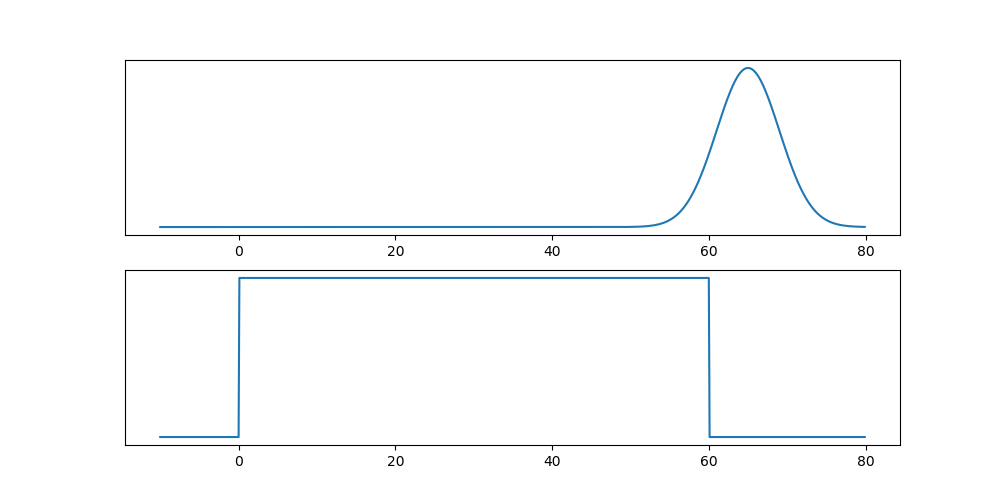
\includegraphics[width=1.0\textwidth]{distributions.png}
\caption{A normal, and uniform, distributions, shown as KDE-like curves.}
\label{distributions}
\end{figure}

If you're interpreting Figure~\ref{distributions} correctly, you can see that
if we generate random numbers from the top distribution, the majority will be
between 60-ish and 70-ish miles per hour, with many near 65 mph and almost
never anything lower than 50 or greater than 80. If we generate them from the
bottom distribution, however, the babies' birth minutes will all be between 0
and 60 but with no particular tendency towards any value in that range more
than any other.

\subsection{Generating normal random numbers}

\index{normal random value}
\index{normal@\texttt{normal()} (NumPy)}

Let's see if that works. The three arguments to \texttt{normal()} are (1) the
mean of the distribution, (2) the standard deviation, and (3) how many random
numbers you actually want. We'll just start with one at a time:

\begin{Verbatim}[fontsize=\small,samepage=true,frame=single,framesep=3mm]
np.random.seed(13)
print(np.random.normal(65,4,1))
\end{Verbatim}
\vspace{-.2in}

\begin{Verbatim}[fontsize=\small,samepage=true,frame=leftline,framesep=5mm,framerule=1mm]
[62.15043735]
\end{Verbatim}

\begin{Verbatim}[fontsize=\small,samepage=true,frame=single,framesep=3mm]
print(np.random.normal(65,4,1))
\end{Verbatim}
\vspace{-.2in}

\begin{Verbatim}[fontsize=\small,samepage=true,frame=leftline,framesep=5mm,framerule=1mm]
[68.01506551]
\end{Verbatim}

\begin{Verbatim}[fontsize=\small,samepage=true,frame=single,framesep=3mm]
print(np.random.normal(65,4,1))
\end{Verbatim}
\vspace{-.2in}

\begin{Verbatim}[fontsize=\small,samepage=true,frame=leftline,framesep=5mm,framerule=1mm]
[64.82198769]
\end{Verbatim}

\begin{Verbatim}[fontsize=\small,samepage=true,frame=single,framesep=3mm]
print(np.random.normal(65,4,1))
\end{Verbatim}
\vspace{-.2in}

\begin{Verbatim}[fontsize=\small,samepage=true,frame=leftline,framesep=5mm,framerule=1mm]
[66.80724935]
\end{Verbatim}

True to form. We keep getting numbers quite close to 65 mph, with a little bit
of variation. Note that if we reset the seed to our original value, our next
call to \texttt{normal()} gives an identical result to the first one, above:

\begin{Verbatim}[fontsize=\small,samepage=true,frame=single,framesep=3mm]
np.random.seed(13)
print(np.random.normal(65,4,1))
\end{Verbatim}
\vspace{-.2in}

\begin{Verbatim}[fontsize=\small,samepage=true,frame=leftline,framesep=5mm,framerule=1mm]
[62.15043735]
\end{Verbatim}

And of course it's easy to generate many speeds at a time (say, eight):

\begin{Verbatim}[fontsize=\small,samepage=true,frame=single,framesep=3mm]
print(np.random.normal(65,4,8))
\end{Verbatim}
\vspace{-.2in}

\begin{Verbatim}[fontsize=\small,samepage=true,frame=leftline,framesep=5mm,framerule=1mm]
[60.81849148 61.8440439  59.95357622 67.25138714 64.02669499 68.65496282
 66.26940369 65.50921312]
\end{Verbatim}

Notice that each time we call \texttt{normal()}, we get an array back (even if
it has only a single value).

By the way, we should sure expect that if we generate many random speeds, and
take their average, it should be pretty darn close to 65 mph:

\begin{Verbatim}[fontsize=\small,samepage=true,frame=single,framesep=3mm]
print(np.random.normal(65,4,1000).mean())                        
\end{Verbatim}

\begin{Verbatim}[fontsize=\small,samepage=true,frame=leftline,framesep=5mm,framerule=1mm]
65.01577962051226
\end{Verbatim}

Yep.

\subsection{Generating uniform random numbers}

\index{uniform random value}
\index{uniform@\texttt{uniform()} (NumPy)}

Uniform random values can be generated the same way, but with the
\texttt{uniform()} function, which takes as its arguments (1) the min, (2) the
max, and (3) the number of desired values:

\begin{Verbatim}[fontsize=\small,samepage=true,frame=single,framesep=3mm]
np.random.seed(13)
print(np.random.uniform(0,60,1))
\end{Verbatim}
\vspace{-.2in}

\begin{Verbatim}[fontsize=\small,samepage=true,frame=leftline,framesep=5mm,framerule=1mm]
[46.66214463]
\end{Verbatim}

This synthetic baby was born at 46.6 minutes past the hour. What about the next
one?


\begin{Verbatim}[fontsize=\small,samepage=true,frame=single,framesep=3mm]
print(np.random.uniform(0,60,1))
\end{Verbatim}
\vspace{-.2in}

\begin{Verbatim}[fontsize=\small,samepage=true,frame=leftline,framesep=5mm,framerule=1mm]
[14.2524732]
\end{Verbatim}

And the next one?

\begin{Verbatim}[fontsize=\small,samepage=true,frame=single,framesep=3mm]
print(np.random.uniform(0,60,1))
\end{Verbatim}
\vspace{-.2in}

\begin{Verbatim}[fontsize=\small,samepage=true,frame=leftline,framesep=5mm,framerule=1mm]
[49.45671196]
\end{Verbatim}

And the next eleven?

\begin{Verbatim}[fontsize=\small,samepage=true,frame=single,framesep=3mm]
print(np.random.uniform(0,60,11))
\end{Verbatim}
\vspace{-.2in}

\begin{Verbatim}[fontsize=\small,samepage=true,frame=leftline,framesep=5mm,framerule=1mm]
[57.94495188 58.35606683 27.20695485 36.54254777 46.53159088 38.49680069
 43.32109377  2.10219145 17.90696825  3.51074951 51.42365656]
\end{Verbatim}

Of course, resetting the seed gives us our original sequence back:

\begin{Verbatim}[fontsize=\small,samepage=true,frame=single,framesep=3mm]
print(np.random.uniform(0,60,5))
\end{Verbatim}
\vspace{-.2in}

\begin{Verbatim}[fontsize=\small,samepage=true,frame=leftline,framesep=5mm,framerule=1mm]
[46.66214463 14.2524732  49.45671196 57.94495188 58.35606683]
\end{Verbatim}

(Check those numbers with the previous ones to convince yourself.)

And finally, let's sanity check the average:

\begin{Verbatim}[fontsize=\small,samepage=true,frame=single,framesep=3mm]
print(np.random.uniform(0,60,1000).mean())                       
\end{Verbatim}
\vspace{-.2in}

\begin{Verbatim}[fontsize=\small,samepage=true,frame=leftline,framesep=5mm,framerule=1mm]
29.2049841447296
\end{Verbatim}

Yay. ``On average,'' our thousand synthetic babies are born at about half past
the hour, which is what we'd expect.


\section{Generating categorical random values}

\index{random value}
\index{categorical random value}
\index{choice@\texttt{choice()} (NumPy)}

NumPy also provides a way to generate \textit{categorical} values with certain
frequencies, through its \texttt{choice()} function. You give it an array of
the possible values, and it chooses one:

\begin{Verbatim}[fontsize=\small,samepage=true,frame=single,framesep=3mm]
np.random.seed(13)
np.random.choice(['Steelers','Redskins','Giants'])
\end{Verbatim}
\vspace{-.2in}

\begin{Verbatim}[fontsize=\small,samepage=true,frame=leftline,framesep=5mm,framerule=1mm]
'Giants'
\end{Verbatim}

\begin{Verbatim}[fontsize=\small,samepage=true,frame=single,framesep=3mm]
np.random.choice(['Steelers','Redskins','Giants'])
\end{Verbatim}
\vspace{-.2in}

\begin{Verbatim}[fontsize=\small,samepage=true,frame=leftline,framesep=5mm,framerule=1mm]
'Steelers'
\end{Verbatim}

(As always, resetting the seed will restart the same sequence of random team
choices from the beginning.)

\pagebreak
\begin{samepage}
Other useful arguments to \texttt{choice()} include:

\begin{compactitem}
\item \texttt{size} -- the number of elements you want in the resulting array.
\item \texttt{replace} -- if \texttt{False}, the elements will be drawn from
your list \textit{without replacement} (meaning once a value is chosen, it
will not be chosen again). This is often useful.
\item \texttt{p} -- a list of \textit{probabilities} (in the range 0 to 1)
specifying how likely each element in the list is to be chosen. (Note these
must sum to 1; and NumPy, stupidly, will not normalize it for you.)
\end{compactitem}
\end{samepage}

To illustrate:

\begin{Verbatim}[fontsize=\footnotesize,samepage=true,frame=single,framesep=3mm]
print(np.random.choice(['Steelers','Redskins','Giants'], size=14, p=[.3,.6,.1]))
\end{Verbatim}
\vspace{-.2in}

\begin{Verbatim}[fontsize=\footnotesize,samepage=true,frame=leftline,framesep=5mm,framerule=1mm]
['Steelers' 'Redskins' 'Redskins' 'Redskins' 'Giants' 'Steelers' 'Steelers'
 'Redskins' 'Redskins' 'Steelers' 'Redskins' 'Giants' 'Steelers' 'Redskins']
\end{Verbatim}

We asked for 14 random teams, and we told it to give us \texttt{Steelers} 30\%
of the time, \texttt{Redskins} 60\%, and \texttt{Giants} only 10\%. I think
you'll agree that the resulting array was pretty faithful to that. (Of course,
you'll get a different random array each time.)

Finally, let's test a large random array and verify that the requested
percentages are approximately correct:

\begin{Verbatim}[fontsize=\small,samepage=true,frame=single,framesep=3mm]
pd.Series(np.random.choice(['Steelers','Redskins','Giants'], size=1000,
    p=[.3,.6,.1])).value_counts() 
\end{Verbatim}
\vspace{-.2in}

\begin{Verbatim}[fontsize=\small,samepage=true,frame=leftline,framesep=5mm,framerule=1mm]
Redskins    584
Steelers    319
Giants       97
dtype: int64
\end{Verbatim}

\index{value\_counts@\texttt{.value\_counts()} (Pandas)}

Our friend the \texttt{.value\_counts()} method confirms that it pretty much
checks out.


